\pdfoutput=1
\documentclass[paper,twocolumn]{geophysics}
%\documentclass[manuscript]{geophysics}
%\documentclass[manuscript,endfloat]{geophysics}
%\documentclass[twocolumn]{article}
\usepackage{natbib}
\usepackage{graphicx}
\usepackage{amsmath}
\usepackage{hyperref}
\newcommand{\mitbf}[1]{\mathbf{{#1}}}

% To leave comments
\usepackage[colorinlistoftodos]{todonotes}


\hypersetup{
    colorlinks=true,
    citecolor=blue,
    linkcolor=blue,
    urlcolor=blue,
    pdfauthor={Uieda et al.},
    pdftitle={Tesseroids: forward modeling gravitational fields in spherical
              coordinates}
}
\title{
    Tesseroids: forward modeling gravitational fields in spherical coordinates
}
\author{
    Leonardo Uieda\footnotemark[1]\footnotemark[2],
    et al.
}


\begin{document}

\maketitle

\righthead{Tesseroids}
\ms{Submission} % manuscript number

\address{
    \noindent
    \footnotemark[1]Universidade do Estado do Rio de Janeiro,
    Rio de Janeiro, Brazil.
    email: leouieda@gmail.com
    \footnotemark[2]Observat\'orio Nacional,
    Rio de Janeiro, Brazil.
}

\begin{abstract}
\end{abstract}

%%%%%%%%%%%%%%%%%%%%%%%%%%%%%%%%%%%%%%%%%%%%%%%%%%%%%%%%%%%%%%%%%%%%%%%%%%%%%%
\section{Introduction}


\todo[inline]{Here's a comment!}

Satellite missions dedicated to measuring the Earths gravity field
(like CHAMP, GRACE, and GOCE)
have provided geophysicists with almost uniform and global data coverage.
These new data have enabled interpretations on regional and global scales
\citep[e.g.][]{Reguzzoni2013,Braitenberg2015}.
Modeling at such scales requires taking into account the curvature of the
Earth and calculating gravity gradients as well as the traditional
gravitational acceleration.
A common approach to achieve this is
to discretize the Earth into tesseroids (Figure~\ref{fig:tesseroid})
instead of rectangular prisms.
However, the integral formula for the gravitational effects of a tesseroid
must be solved numerically.
Approaches to this numerical integration include
Taylor series expansion \citep{Heck2007, Grombein2013}
and the Gauss-Legendre Quadrature \citep{Asgharzadeh2007}.
Taylor series expansion produces accurate results at low latitudes but
presents a decrease in accuracy towards the polar regions.
This is attributed to tesseroids degenerating into an approximately triangular
shape at the poles.
The Gauss-Legendre Quadrature (GLQ) integration consists of approximating
the volume integral by a weighted sum of the effect of point masses.
An advantage of the GLQ approach is that the accuracy of integration can be
controlled by the number of point masses used.
A disadvantage is the increased computation time as the number of
point masses increases.
Thus, there is a trade-off between accuracy and computation time, a common
theme in numerical methods.
\citet{Wild-Pfeiffer2008} investigated the use of different mass elements,
including tesseroids, to compute the gravitational effects of topographic
masses.
The author concludes that using tesseroids with GLQ integration gives the best
results for near-zone computations.
However, the question of how to determine the optimal parameters for GLQ
integration remained open.


Previous work by \citet{Ku1977} investigated the use of the Gauss-Legendre
Quadrature in gravity forward modeling.
\citet{Ku1977} numerically integrated the vertical component of the
gravitational acceleration of right rectangular prisms.
The author suggested that the accuracy of the GLQ integration depends on
the ratio between distance to the computation point and the distance between
adjacent point masses.
Based on this, \citet{Ku1977} proposed an empirical criteria that the distance
between adjacent point masses should be less than the distance to the computation point.
\citet{Asgharzadeh2007} proposed using this criteria for the GLQ integration of
the gravity gradient tensor of tesseroids.
To our knowledge, there has been no investigation if the empirical criteria of
\citet{Ku1977} is valid for gravity gradient components or for tesseroids.
There has also been no attempt to quantify the error committed in the GLQ
integration when applying the criteria of \citet{Ku1977}.


\citet{Li2011} devised an algorithm to automatically enforce the criteria of
\citet{Ku1977}.
Their algorithm divides the tesseroid into smaller ones instead of increasing
the number of point masses per tesseroid.
This division effectively increases the total number of point masses
because the number of points masses per tesseroid is fixed.
The criterion used decide if a division is necessary is
that the minimum distance to the computation point must be larger than
the largest dimension of the tesseroid.
This division is repeated recursively until all tesseroids obey the criteria.
Then, GLQ integration is performed for each of the smaller tesseroids
using the specified number of point masses.
The advantage of this adaptive discretization over
increasing the number of points masses is that the
total total distribution of point masses will be greater
only close to the computation point.
This makes the adaptive discretization more computationally efficient.


\citet{Grombein2013} developed optimized formula for the gravitational fields
of tesseroids using Cartesian integral kernels.
These formula are faster to compute and don't have singularities at the poles
like their spherical counterparts.
The Cartesian formula are numerically integrated using a Taylor series
expansion as per \citet{Heck2007}.
\citet{Grombein2013} use a near-zone separation to mitigate the increased error
at high latitudes.
In the so called ``near-zone'' of the computation point they use a finner
discretization with smaller tesseroids.
This is accomplished by dividing the tesseroids along their horizontal
dimensions.
However, the determination of an optimal size of the near-zone remains an
open question \citep{Grombein2013}.


We have implemented a modified version of the adaptive discretion of
\citet{Li2011} into the open-source software package \textit{Tesseroids}.
The software uses the Cartesian formula of \citet{Grombein2013} for improved
performance and robustness.
Previous versions of \textit{Tesseroids} have been used by, e.g.,
\citet{Alvarez2012, Bouman2013, Bouman2013a, Mariani2013, Braitenberg2014,
Braitenberg2011, Fullea2014}.
This article describes the software \textit{Tesseroids} and the implementation
of our modified adaptive discretization algorithm.
We also present a numerical investigation of the error committed
in the computations.
These results allow us calibrate the adaptive discretization algorithm
separately for the gravitational potential, gravitational acceleration,
as well as the gravity gradient tensor components.


%%%%%%%%%%%%%%%%%%%%%%%%%%%%%%%%%%%%%%%%%%%%%%%%%%%%%%%%%%%%%%%%%%%%%%%%%%%%%%
\section{Theory}


\begin{figure}
    \centering
    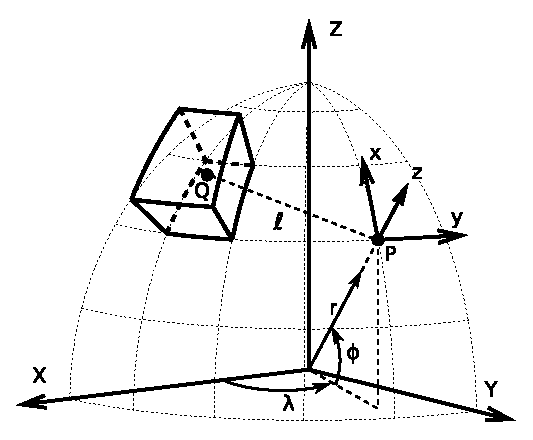
\includegraphics[width=0.4\textwidth]{figs/tesseroid}
    \caption{
        View of a tesseroid,
        the integration point $Q$ inside the tesseroid,
        a geocentric coordinate system $(X, Y, Z)$,
        the computation $P$ and it's local coordinate system $(x, y, z)$.
        $r$, $\phi$, $\lambda$ are
        the radius, latitude, and longitude, respectively, of point $P$,
        and $\ell$ is the Cartesian distance between $P$ and $Q$.
    }
    \label{fig:tesseroid}
\end{figure}

A tesseroid is a mass element defined in geocentric spherical
coordinates
(Figure~\ref{fig:tesseroid}).
It is bounded by two meridians, two parallels, and two concentric circles.
The gravitational fields of a tesseroid at a point $P = (r,\phi,\lambda)$
are determined with respect to the local North-oriented coordinate system at
P (x, y, z in Figure~\ref{fig:tesseroid}).
\citet{Grombein2013} formulated Cartesian kernels for the volume integrals
that define the tesseroid gravitational potential, gravitational attraction,
and Marussi tensor, respectively,

\begin{equation}
    V(r,\phi,\lambda) = G \rho
        \int\limits_{\lambda_1}^{\lambda_2}
        \int\limits_{\phi_1}^{\phi_2}
        \int\limits_{r_1}^{r_2}
        \frac{1}{\ell}
        \kappa\  dr^\prime d\phi^\prime d\lambda^\prime,
    \label{eq:tesspot}
\end{equation}
\begin{equation}
    g_{\alpha}(r,\phi,\lambda) = G \rho
        \int\limits_{\lambda_1}^{\lambda_2}
        \int\limits_{\phi_1}^{\phi_2}
        \int\limits_{r_1}^{r_2}
        \frac{\Delta_\alpha}{\ell^3}
        \kappa\ dr^\prime d\phi^\prime d\lambda^\prime,
    \label{eq:tessgrav}
\end{equation}
\noindent
and
\begin{equation}
    g_{\alpha\beta}(r,\phi,\lambda) = G \rho
        \int\limits_{\lambda_1}^{\lambda_2}
        \int\limits_{\phi_1}^{\phi_2}
        \int\limits_{r_1}^{r_2}
        I_{\alpha\beta}
        \ \kappa\ dr^\prime d\phi^\prime d\lambda^\prime.
    \label{eq:tesstensor}
\end{equation}
\begin{equation}
    I_{\alpha\beta} =
    \left(
        \frac{3\Delta_{\alpha} \Delta_{\beta}}{\ell^5} -
        \frac{\delta_{\alpha\beta}}{\ell^3}
    \right)
    \label{eq:tesstensorkernel}
\end{equation}

\noindent
where $\alpha, \beta \in \{x, y, z\}$,
$\rho$ is the density,
$G = 6.673\times10^{-11}\ m^3kg^{-1}s^{-1}$ is the gravitational constant,
and

\begin{equation}
    \Delta_x = r^\prime(\cos\phi\sin\phi^\prime - \sin\phi\cos\phi^\prime
               \cos(\lambda^\prime - \lambda)),
\end{equation}
\begin{equation}
    \Delta_y = r^\prime \cos \phi^\prime \sin(\lambda^\prime - \lambda),
\end{equation}
\begin{equation}
    \Delta_z = r^\prime \cos \psi - r,
\end{equation}
\begin{equation}
    \kappa = {r^\prime}^2 \cos \phi^\prime,
\end{equation}
\begin{equation}
    \ell = \sqrt{{r^\prime}^2 + r^2 - 2 r^\prime r \cos \psi},
\end{equation}
\begin{equation}
    \cos\psi = \sin\phi\sin\phi^\prime + \cos\phi\cos\phi^\prime
                 \cos(\lambda^\prime - \lambda).
\end{equation}

We will follow \citet{Asgharzadeh2007} and perform the numerical integration
using the Gauss-Legendre Quadrature (GLQ).
The GLQ consists of approximating the integral by a weighted sum of the
integration kernel \citep{Hildebrand1987},
\begin{equation}
    \int\limits_a^b f(x) dx \approx
    \frac{b-a}{2}\sum\limits_{i=1}^N W_i f(x_i),
    \label{eq:glq1d}
\end{equation}

\noindent
in which $N$ is the order of the quadrature,
i.e. the number of points used in the GLQ.
The points $x_i$ are called the quadrature nodes.
They are the roots of the $N^{th}$ order Legendre polynomial $P_N(x)$.
For a second order polynomial ($P_2(x)$),
the roots are $x = \pm 0.577350269$.
Roots for larger order polynomials
can be determined by a root finder algorithm.
Roots of Legendre polynomials
will be within the range $[-1, 1]$.
Before being used for GLQ integration,
the roots must be scaled to the integration limits $[a, b]$ using

\begin{equation}
    x^{scaled}_i = \frac{b - a}{2} x_i + \frac{b + a}{2}.
    \label{eq:glq_scaling}
\end{equation}

The weights of the GLQ are given by \citep{Hildebrand1987},

\begin{equation}
    W_i = \frac{2}{(1 - x_i^2)(P^\prime_N(x_i))^2}.
    \label{eq:glq_weights}
\end{equation}

\noindent
The values of $P_N(x)$ and its first derivative $P^\prime_N(x)$
can be calculated with recursive relations.

The Gauss-Legendre Quadrature for three-dimensional volume integrals,
like equations~\ref{eq:tesspot}-\ref{eq:tesstensor},
becomes \citep{Asgharzadeh2007}

\begin{equation}
    \iiint\limits_{\Omega}
    f(r^\prime, \lambda^\prime, \phi^\prime)
    d\Omega
    \approx
    A
    \sum\limits_{i=1}^{N^r}
    \sum\limits_{j=1}^{N^\phi}
    \sum\limits_{k=1}^{N^\lambda}
    f(r_i, \phi_j, \lambda_k),
    \label{eq:glq3d}
\end{equation}

\noindent
where

\begin{equation}
    A = \frac{(\lambda_2 - \lambda_1)(\phi_2 - \phi_1)(r_2 - r_1)}{8}.
\end{equation}

Comparing equation~\ref{eq:glq3d} with
equations~\ref{eq:tesspot}-\ref{eq:tesstensor},
we see that $f(r_i, \phi_j, \lambda_k)$ is the effect of a point
mass located on the quadrature nodes.
Thus, it can be said that the GLQ integration
approximates the volume integrals  by a
weighted sum of point mass effects.

The accuracy of the integration
depends on the number of point masses used in the summation.
\citet{Ku1977} showed that it also depends on the ratio between
the distance to the computation point and the distance between adjacent nodes.
Figure~\ref{fig:glqerrorsample}
illustrates this effect on the $g_{xy}$ gravity gradient component.
The $g_{xy}$ component was produced by a
$7^\circ \times 7^\circ \times 20\ km$ tesseroid
with $2.67\ g.cm^{-3}$ density
and top at $z=0\ km$.
The maps were calculated on a regular grid
with $100\times100$ points.
Figure~\ref{fig:glqerrorsample}a shows the $g_{xy}$ component
calculated at 400 km height using
GLQ with order two ($2 \times 2 \times 2 = 8$ point masses).
Figure~\ref{fig:glqerrorsample}b shows $g_{xy}$ computed with order two
GLQ as well but at 150 km height.
Notice that the computed effect is concentrated around each point mass
of the GLQ (black dots) and does not resemble the effect of a tesseroid.
\citet{Ku1977} determined an empirical criterion that the distance between
point masses (quadrature nodes) should be smaller than the minimum distance to
the computation point.
Thus, if a computation point is too close to the tesseroid one would have to
decrease the distance between the point masses in order to obtain an accurate
result.
One way to accomplish this would be increase the order of the quadrature
$N$ in all three directions.
Figure~\ref{fig:glqerrorsample}c shows the $g_{xy}$ component calculated at
150km height but with a GLQ order of 30
($30 \times 30 \times 30 = 27,000$ point masses).
The computed $g_{xy}$ component more closely resembles
the expect results for a single tesseroid \citep{Asgharzadeh2007}.

\begin{figure}
    \centering
    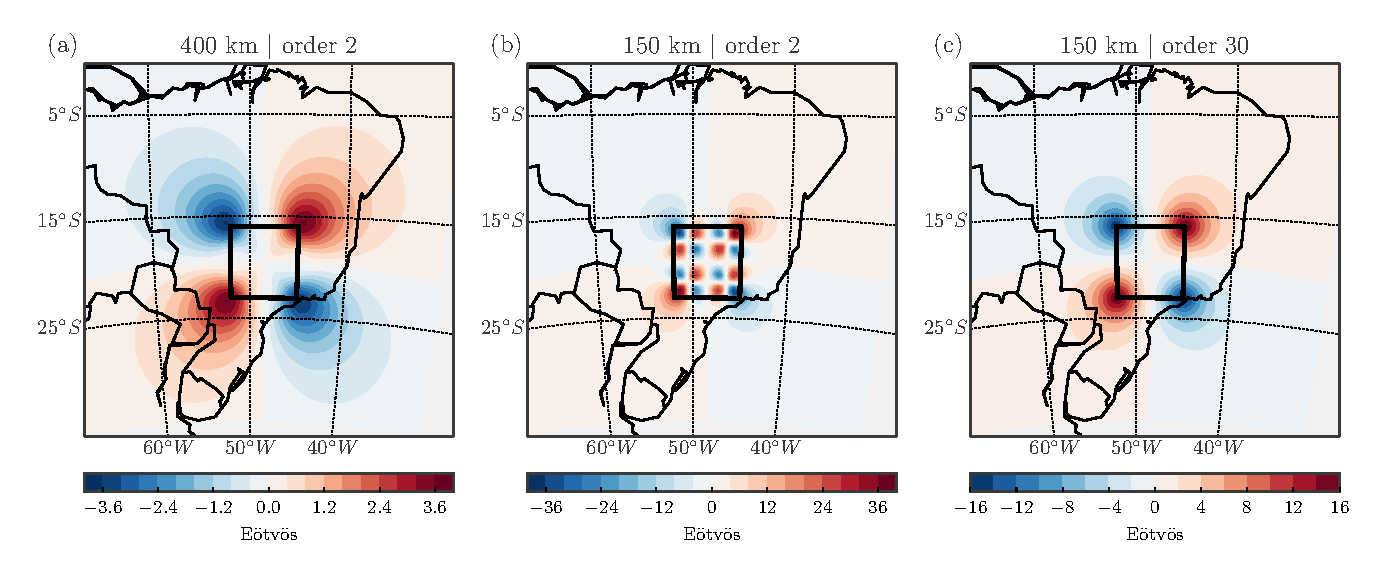
\includegraphics[width=0.4\textwidth]{figs/vary-height-and-order}
    \caption{
        Example of the effect of varying
        the computation height
        and the number of point masses in the Gauss-Legendre Quadrature.
        Black circles represent the horizontal location of the point masses.
        a) $g_{xy}$ calculated at $400\ km$ height using GLQ order 2
        ($2 \times 2 \times 2 = 8$ point masses).
        b) At $150\ km$ height and GLQ order 2,
        the result resembles that of
        four point mases instead of a single tesseroid.
        This effect was shown by \citet{Ku1977}.
        c) At $150\ km$ but with a higher GLQ order of 30,
        the result is similar to that expected for a single mass source.
    }
    \label{fig:glqerrorsample}
\end{figure}


\subsection{Adaptive discretization}

\citet{Li2011} proposed an alternative method
for decreasing the distance between point masses
and achieve an accurate integration.
Instead of increasing the GLQ order,
they keep it fixed to a given number
and divide the tesseroid into smaller parts.
The sum of the effects of the smaller tesseroids
is equal to the gravitational effect of the larger tesseroid.
This division effectively decreases
the distance between nodes because
of the smaller size of the tesseroids.
The criterion for dividing a tesseroid or not
is that the distance to the computation point
must be smaller than a constant times the size of the tesseroid.
This is analogous to the criterion of \citet{Ku1977}
because the size of the tesseroid serves as a proxy
for the distance between point masses.
This procedure is repeated recursively
(i.e., to each of the smaller tesseroids and so on)
until all tesseroids are within the acceptable
ratio of distance and size or a minimum size is achieved.


The advantage of this adaptive discretization is
that the number of point masses is only increased
in regions of the tesseroid that are
closer to the computation point.
Alternatively,
simply increasing the order of the GLQ
would increase the number of point masses
evenly throughout the whole tesseroid.

%%%%%%%%%%%%%%%%%%%%%%%%%%%%%%%%%%%%%%%%%%%%%%%%%%%%%%%%%%%%%%%%%%%%%%%%%%%%%%
\section{Implementation}

We have implemented the calculation of
the tesseroid gravitational fields
with adaptive discretization
in the open-source package \textit{Tesseroids}.
It is freely available
online through the software website\footnote{
\href{http://tesseroids.leouieda.com}{http://tesseroids.leouieda.com}}
under the BSD 3-clause open-source license.
An archived version of the source code
is available as part of this article
and online\footnote{\href{}{\todo[inline]{insert a ZENODO doi}}}.

\textit{Tesseroids}  consists of command-line programs
written in the C programming language.
The package includes programs to calculate
the gravitational fields of tesseroids and
rectangular prisms (in both Cartesian and spherical coordinates),
as well as model and computation grid generation.
All programs receive input through
command-line arguments and the standard input channel (STDIN)
and output the results through the standard output channel (STDOUT).
For example,
the command to generate a regular grid with $NLON \times NLAT$ points,
calculate on it $g_z$ and $g_{zz}$ caused by
the tesseroids in a file ``MODELFILE'',
and save the results to a file called ``OUTPUT''
is:

\begin{verbatim}
tessgrd -rW/E/S/N -bNLON/NLAT -zHEIGHT | \
    tessgz MODELFILE | \
    tessgzz MODELFILE > OUTPUT
\end{verbatim}

The \texttt{src} folder of the source code archive
contains the C files that build the command-line programs
(e.g., \texttt{tessgz.c}).
The \texttt{src/lib} folder contains
the source files that implement the numerical computations.
We will not describe here the implementation of the input/output parsing and
other miscellanea.
Instead, we will focus on the details of the Gauss-Legendre Quadrature
integration of equations~\ref{eq:tesspot}-\ref{eq:tesstensor}
and the adaptive discretization of tesseroids.



\subsection{Numerical integration}

The source file \texttt{src/lib/glq.c}
contains the code necessary to perform
a Gauss-Legendre Quadrature integration.
The first step in the GLQ is to compute the
locations of the discretization points (i.e., the point masses).
These points are roots of Legendre polynomials.
Precomputed values are available low order polynomials,
typically up to order five.
For flexibility and to compute higher order roots,
we use the multiple root-finder algorithm of
\citet{Barrera-Figueroa2006}.
The additional computational load is minimal
because the root-finder algorithm
must be run only once per program execution.
The root-finder is implemented in functions
\texttt{glq\_nodes} and \texttt{glq\_next\_root}.
The computed roots will be in the range $[-1, 1]$
and must be scaled to the integration limits
(the physical boundaries of the tesseroid)
using function \texttt{glq\_set\_limits} (see equation~\ref{eq:glq_scaling}).

The GLQ weights (equation~\ref{eq:glq_weights})
are computed by function \texttt{glq\_weights}.
Both the computed roots and weights are stored in a data structure
(a C \texttt{struct}) called \texttt{GLQ}.
Function \texttt{glq\_new}
handles memory allocation,
calculates the roots and weights,
and returns the complete \texttt{GLQ} structure.

The numerical integration of the tesseroid gravitational fields
is performed by the functions in module \texttt{src/lib/grav\_tess.c}.
Functions \texttt{tess\_pot}, \texttt{tess\_gx}, \texttt{tess\_gy}, and so on,
compute the gravitational fields of a single tesseroid
on a single computation point.
These functions require three \texttt{GLQ} structures,
each containing the roots and weights
for GLQ integration in the three dimensions.
The roots must be scaled to the
integration limits
$[\lambda_1, \lambda_2], [\phi_1, \phi_2], [r_1, r_2]$
(see equations~\ref{eq:tesspot}-\ref{eq:tesstensor}).
The integration consists of three loops
that sum the weighted kernel functions
evaluated at each GLQ point mass (the scaled roots).

The biggest bottlenecks for the numerical integration are
the number of point masses used
and the evaluation of the trigonometric functions in
equations~\ref{eq:tesspot}-\ref{eq:tesstensor} inside the inner loops.
Better performance is achieved
by pre-computing the sine and cosine of latitudes
and moving some trigonometric function evaluations
to the outer loops.


\subsection{Implementation of adaptive discretization}

Our implementation of the adaptive discretization algorithm
differs in a few ways from the original.
In \citet{Li2011},
a tesseroid will be divided when
the smallest distance between it and the computation point
is smaller than a constant times
the largest dimension of the tesseroid.
Instead of the smallest distance,
we use the easier to calculate
distance between
the computation point $(r, \lambda, \phi)$
and the geometric center of the tesseroid
$(r_t, \lambda_t, \phi_t)$

\begin{equation}
    d = \left[
        r^2 + r_t^2 - 2 r r_t \cos\psi_t
        \right]^{\frac{1}{2}}.
    \label{eq:distance}
\end{equation}
\begin{equation}
    \cos\psi_t =
        \sin\phi\sin\phi_t + \cos\phi\cos\phi_t\cos(\lambda - \lambda_t)
\end{equation}

Our definition of the dimensions of the tesseroid
(the ``side lengths'' of \citet{Li2011})
along longitude, latitude, and radius, respectively, are
(Figure~\ref{fig:division}a)

\begin{equation}
    L_\lambda = r_2 \arccos(\sin^2\phi_t +
        \cos^2\phi_t\cos(\lambda_2 - \lambda_1)),
    \label{eq:sizelon}
\end{equation}
\begin{equation}
    L_\phi = r_2 \arccos(\sin\phi_2\sin\phi_1 + \cos\phi_2\cos\phi_1),
\end{equation}
\begin{equation}
    L_r = r_2 - r_2.
    \label{eq:sizer}
\end{equation}

\noindent
$L_\lambda$ and $L_\phi$ are arc-distances measured along the top surface of
the tesseroid (Figure~\ref{fig:division}a).
Specifically, $L_\lambda$ is measured long the middle latitude of the
tesseroid ($\phi_t$).

To determine if a tesseroid must be divided,
we check if

\begin{equation}
    \frac{d}{L_i} < D,
    \label{eq:condition}
\end{equation}

\noindent
for each $i \in (\lambda, \phi, r)$.
$D$ is a positive scalar
hereafter referred to as the ``distance-size ratio''.
If the inequality holds for all three dimensions,
the tesseroid is not divided.
Thus, the distance-size ratio determines
how close the computation point can be
before we must divide the tesseroid.
The value of $D$ is indirectly responsible for
the accuracy of the solution and the computation time.
We will explore the relationship with the accuracy in the following section.

Figure~\ref{fig:division} shows examples of
the resulting tesseroid models after adaptive discretization.
Figure~\ref{fig:division}a shows
the initial tesseroid and computation point P.
Figures~\ref{fig:division}b-d are
the result of adaptive discretization using
different values of the distance-size ratio $D$,
respectively,
$D=1$, $D=2$, and $D=6$.
The number of tesseroids in the resulting discretization is, respectively,
4, 38, and 936.

\begin{figure}
    \centering
    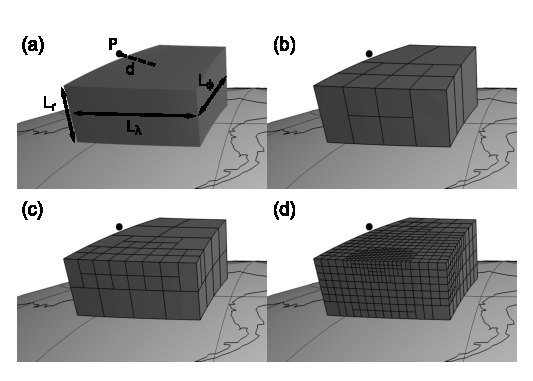
\includegraphics[width=0.4\textwidth]{figs/tesseroid-split}
    \caption{
        Adaptive discretization
        of the tesseroid shown in (a)
        for a computation point P
        using the distance-size ratio $D$ equal to
        (b) 1, (c) 2, and (d) 6.
        $d$ is the Cartesian distance between
        the center of the top face of the tesseroid
        and $P$.
        $L_r$, $L_\phi$, and $L_\lambda$ are the dimensions of the tesseroid.
        Note that increasing $D$
        results in a fine division of the tesseroid
        close the computation point
        and a coarser division further away.
    }
    \label{fig:division}
\end{figure}

Instead of using recursive function calls,
as originally proposed by \citet{Li2011},
we use a stack-based implementation of the algorithm.
Stacks are array-like data structures
with a particular way of inserting and removing elements from it.
In a stack,
one can only insert elements to the top of the stack
(the last empty position).
Likewise,
one can only remove the last element of the stack
(commonly referred to as ``popping'' the stack).
Stacks are also known as ``Last-in-first-out'', or LIFO, data structures.

We will describe the stack-based algorithm
for computing the effect of a single tesseroid
on a single computation point.
The algorithm is implemented in function \texttt{calc\_tess\_model\_adapt}
of the file \texttt{src/lib/grav\_tess.c}.
The stack of tesseroids is represented by
the \texttt{stack} variable,
an array of \texttt{TESSEROID} structures.
We must define a maximum size for the stack to allocate memory for it.
Defining a maximum size allows us to
avoid an infinite loop
in case the computation point is on
(or sufficiently close to) the surface of the tesseroid.
We use the integer \texttt{stktop}
to keep track of the index of
the last element in the stack (the top of the stack).

The algorithm starts by creating an empty stack of tesseroids.
Then, the stack is initialized with the input tesseroid.
The initialization is done by copying the tesseroid into the stack
and setting \texttt{stktop} to zero (the first element).
Once the stack is initialized, the steps of the algorithm are:

\begin{enumerate}
    \item ``Pop'' the stack (i.e., take the last tesseroid from it).
        This will cause \texttt{stktop} to be reduced by one.
        This tesseroid is the one that will be evaluated in the following
        steps.
    \item Compute the distance $d$ between
        the geometric center of the tesseroid and
        the computation point using equation~\ref{eq:distance}.
    \item Compute the dimensions of the tesseroid $L_\lambda$, $L_\phi$,
        and $L_r$ using equations~\ref{eq:sizelon}-\ref{eq:sizer}.
    \item Check the condition in equation~\ref{eq:condition} for each
        dimension of the tesseroid.
    \item If none of the dimensions fail the above condition,
        compute the gravitational effect of the tesseroid using the
        Gauss-Legendre Quadrature
        (equations~\ref{eq:tesspot}-\ref{eq:tesstensor} and~\ref{eq:glq3d}).
        We use a GLQ order of two for all three dimensions
        ($2 \times 2 \times 2 = 8$ point masses)
        by default.
        This value can be changed using
        a command-line argument of the modeling programs.
    \item If any of the dimensions fail the condition:
    \begin{enumerate}
        \item Divide the tesseroid in half along each dimension that failed
             the condition.
        \item Check if the number of new elements plus \texttt{stktop}
             is smaller than the maximum stack size.
             If it is not (i.e., the stack is full),
             warn the user of a ``stack overflow''
             and compute the effect of the larger tesseroid (step 5).
        \item If the stack is not full, place the smaller tesseroids into
             the stack.
    \end{enumerate}
    \item Repeat the above steps until the stack is empty
        (\texttt{stktop} is equal to -1).
\end{enumerate}

This stack-based implementation
has some advantages over the original recursive implementation,
namely:
(1) It will be faster because it bypasses the overhead of function calls.
(2) It gives the developer more control over the recursion step.
In recursive implementations,
the developer has no control over
the maximum number of consecutive recursive calls
(i.e., the ``recursion depth'').
This limit may vary with programming language,
compiler, and operating system.
Overflowing the maximum recursion depth
may result in program crashes,
typically with cryptic or inexistent error messages.
In the stack-based implementation,
the developer has complete control.
Overflowing of the stack can be handled gracefully
with an error message
or even performing a suitable approximation of the result.

\subsection{Reproducing analysis and results}


All figures and numerical experiments in this article
were produced in IPython notebooks\footnote{
\href{http://ipython.org}{http://ipython.org}}
\citep{Perez2007}.
These files combine the analysis and figure generation source code
with text, equations, and the figures generated by the code.
We used \textit{pandas} by \citet{Mckinney2010}
to perform the data analysis,
\textit{matplotlib} by \citet{Hunter2007} for graphs,
and \textit{Mayavi} by \citet{Ramachandran2011} for 3D graphs.

The notebook files,
as well as instructions for installing and running the analysis,
are distributed along with the source code archive
that accompanies this article.
Alternatively,
all accompanying material can be downloaded
from an online source code repository\footnote{
\href{https://github.com/pinga-lab/paper-tesseroids}{https://github.com/pinga-lab/paper-tesseroids}}
or a persistent archive\footnote{
\href{}{\todo[inline]{Replace with the Zenodo/figshare DOI for the repo.}}}.



%%%%%%%%%%%%%%%%%%%%%%%%%%%%%%%%%%%%%%%%%%%%%%%%%%%%%%%%%%%%%%%%%%%%%%%%%%%%%%
\section{Evaluation of the accuracy}

The key controlling point of the adaptive discretization algorithm
is the distance-size ratio $D$ (equation~\ref{eq:condition}).

$D$ indirectly controls both the accuracy of the integration
and the computation time.

The specific value chosen for $D$ determines how many divisions will be made
(Figure~\ref{fig:division}).

\citet{Li2011} provide a few examples of values for this ratio in the case of
the vertical component of the gravitational attraction.

In this section, we investigate
the relationship between
values of the distance-size ratio
and the computation error.

We perform the error analysis for the gravitational potential,
acceleration, and gradient tensor components
to evaluate if the same value of $D$ yields compatible error levels
for different fields.



We establish a homogeneous spherical shell as a reference against which to
compare the computed tesseroid fields.

The shell has analytical solutions for the gravitational potential,
attraction, and gradient tensor along the polar axis
\citep{Grombein2013}.

We used a spherical shell with a thickness of 1 km,
density of $2670\ kg.m^{-3}$,
bottom at height 0 km above the reference sphere,
and top at 1 km height.



We discretized the spherical shell along the horizontal dimensions into
a regular mesh of tesseroids.

If we calculate the tesseroid fields at a single point, that point might not
coincide with the point of largest error.

Figure~\ref{fig:glqerrorsample} shows that the largest errors are concentrated
on top of the tesseroid.

Performing the error analysis on calculations at a single point will not be
representative of the true error.

Fortunately, the symmetry of the shell allows us to consider the computation point at any
geographic coordinate.

We calculate the effect of the tesseroid model of the spherical shell
on a regular grid.

The effect of the shell will be same along the entire grid.

We compute the differences between the effects of the shell and the tesseroid
model on the grid and keep only the largest error.

The grid is at a constant height of 2 km (1 km above the shell).

The grid is located on top of a tesseroid located at the North pole.

The computation point can be considered at any point with equal radial
coordinate located outside the shell because of the symmetry of the shell.

We calculate the difference between the shell values and the values computed
from tesseroids.

We keep only the largest difference.

Calculating on a grid above a tesseroid is important because
the largest errors in the GLQ integration occur directly on top of the
tesseroid but not exactly at it's center, as can be seen in
Figure~\ref{fig:glqerrorsample}.

The difference between shell and tesseroid values would be underestimated
if the computation was performed only at a single point on the polar axis.

We repeated the tesseroid calculations with values of the distance-size ratio
$D$ varying from 0 (i.e., no divisions) to 10 in 0.5 intervals.



Figure~\ref{fig:tess_vs_shell} shows the maximum difference between the
shell and tesseroid fields as a function of $D$.

The differences are given as a percentage of the shell value.

The error versus $D$ curves allow us to choose a value of $D$ that
results in an error below a chosen maximum.

We chose 0.1\% as the maximum allowed error.

We performed the computations again for three different scenarios: at 260 km
height (the mean orbit height of the GOCE satellite), on top of a tesseroid at
the equator, and for a $30^\circ \times 30^\circ \times 1\ km$ tesseroid model
of the shell.

We performed these computations to investigate if the GLQ error decays the same
way under different scenarios.

The error curves for the gravitational potential show increased errors at the
equator and for a $30^\circ$ tesseroid.

For $D=1$ all errors are smaller than 0.1\%,
even in the extreme case of a $30^\circ$ tesseroid with computation points at a
height of 1 km above the tesseroid.

$D=1.5$ is sufficient to achieve errors below 0.1\% in $g_z$.

$D=8$ is required to achieve errors below 0.1\% in
the gravity gradient components.

The error curves for the computation at 260 km height shows that
the error is smaller at higher altitudes for all fields.

Computation at 260 km height does not produce errors above the 0.1\% threshold
for the potential and $g_z$.

The computation height changes the value of the distance-size ratio required
for the gravity gradient components.

We computed the error curves for $g_{zz}$ at different heights
(Figure~\ref{fig:gzz_error_height}).

The distance-size ratio can be reduced to 4 if the computation is done at 50 km
height.

One can use a distance-size ratio of 2.5 for computations at 260 km height.

These reductions in the distance-size ratio can reduce the computation time
required to achieve the desired.



The software \textit{Tesseroids} includes default values of the distance-size
ratio.

We used the values required to achieve 0.1\% accuracy: 1 for the potential,
1.5 for the gravitational attraction, and 8 for the gravity gradient
components.

The value of $D=8$ for the gravity gradients is conservative.

We chose it to ensure the accuracy of the computation in most cases.

The experienced user of the software can set smaller values using command-line
options.

The smaller values result in less computation time.

\begin{figure}
    %\centering
    %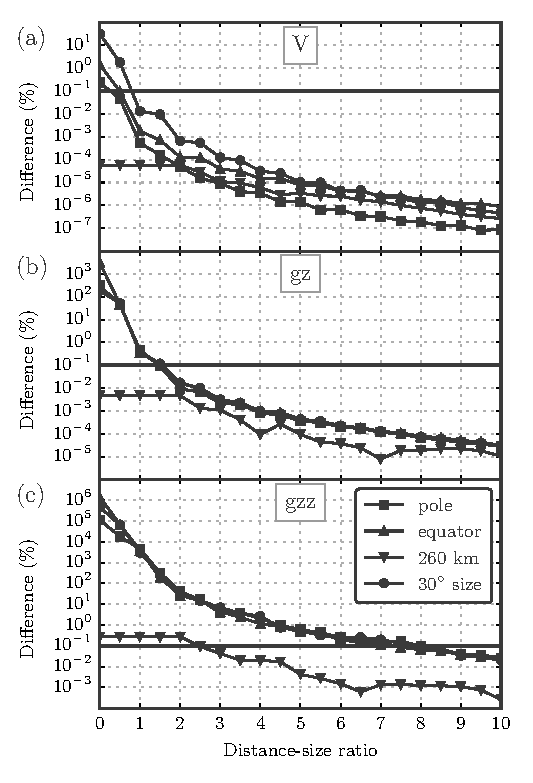
\includegraphics[width=0.4\textwidth]{figs/distance-size-curves}
    \missingfigure{}
    \caption{
        The maximum difference between the computed tesseroid and shell effects
        as a function of the distance-size ratio $D$
        for (a) the gravitational potential, (b) $g_z$, and (c) $g_{zz}$.
        The difference is given as a percentage of the shell effect.
        Curves correspond to the different tesseroid models:
        $1^\circ \times 1^\circ$ tesseroids with computation grid at
        2 km height at the polar region,
        $1^\circ \times 1^\circ$ tesseroids with computation grid at
        2 km height at the equatorial region,
        $1^\circ \times 1^\circ$ tesseroids with computation grid at
        260 km height at the polar region,
        and
        $30^\circ \times 30^\circ$ tesseroids with computation grid at
        2 km height at the polar region.
    }
    \label{fig:dist-size-curves}
\end{figure}

\begin{figure}
    %\centering
    %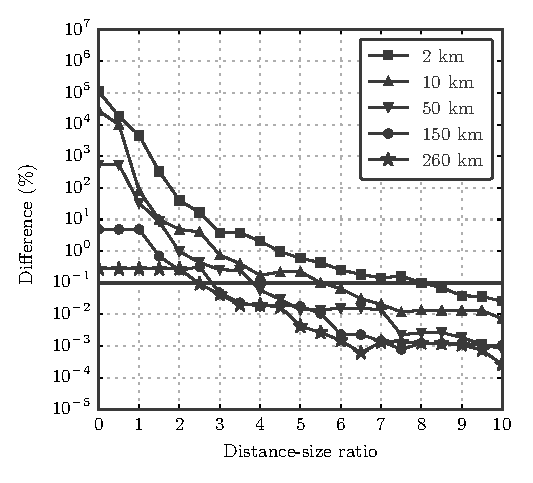
\includegraphics[width=0.4\textwidth]{figs/gzz-with-height}
    \missingfigure{}
    \caption{
        Variation of $g_{zz}$ difference curves for computation grids at
        varying heights.
    }
    \label{fig:gzz-with-height}
\end{figure}


%%%%%%%%%%%%%%%%%%%%%%%%%%%%%%%%%%%%%%%%%%%%%%%%%%%%%%%%%%%%%%%%%%%%%%%%%%%%%%
\section{Conclusions}

%%%%%%%%%%%%%%%%%%%%%%%%%%%%%%%%%%%%%%%%%%%%%%%%%%%%%%%%%%%%%%%%%%%%%%%%%%%%%%
\section{Acknowledgments}


\bibliographystyle{seg}
\bibliography{references.bib}
\end{document}
